\documentclass[10pt,twocolumn]{article}

\usepackage{geometry}
\geometry{
	a4paper,
	left=1cm,
	top=1cm,
	right=1cm,
	bottom=1cm,
}
\usepackage{color}
\usepackage[toc,page]{appendix}
\usepackage{authblk}
\usepackage{amsmath}
\usepackage{url}
\usepackage{graphicx}
\usepackage{float}
\usepackage{listings}
\usepackage{multicol}

\definecolor{mygray}{rgb}{0.4,0.4,0.4}

\lstdefinestyle{cppStyle}{
	captionpos=t,
	numbers=left,
	% xleftmargin=8pt,
	numberstyle=\color{mygray}\ttfamily\small,
	numbersep=8pt,
	language=c++,
	keywordstyle=\color{blue}\small,
	stringstyle=\color{red}\small,
	commentstyle=\color{green}\small,
	basicstyle=\ttfamily\small,
	showstringspaces=false,
	breaklines,
	escapechar=|,
	columns=fullflexible,
}

\pagenumbering{gobble}

\begin{document}

\title{\vspace{-1cm}Bubble Sort using Divide and Conquer with MPI}
\author[1]{Claudio Scheer}
\author[1]{Gabriell Araujo}
\affil[1]{Master's Degree in Computer Science - PUCRS}
\affil[ ]{\textit{\{claudio.scheer, grabriell.araujo\}@edu.pucrs.br}}
\date{}

\maketitle

\section*{General Setup}
We ran our \textit{batch job} on two nodes (2x12 cores, 2x24 when considering hyper-threading) in the Cerrado cluster. All experiments were executed three times and then the average execution time and the standard deviation were calculated. Efficiency and speedup were based on the execution time reported by the sequential execution of the bubble sort algorithm.

For the implementation using MPI, we used the divide and conquer architecture. In short, the unsorted vector is divided until it has a specific size, named delta. The execution forms a perfect balanced binary tree. Therefore, the left and right children of a node sort a part of the vector and send it back to the parent. The parent will merge the two vectors received from the children, maintaining the order of the elements, and sent to the parent, until reaching the master node.

\section*{Bubble Sort}
The bubble sort problem addressed here consists of sorting one vector with 1000000 integers. Figure~\ref{fig:bubble-sort-speedup-efficiency} shows the results of the executions using the sequential (Listing~\ref{lst:bubble-sort-sequential}) and the MPI version (Listing~\ref{lst:bubble-sort-mpi}), with different numbers for delta.

Since only the last level of the execution tree will sort the subvectors, the parent levels will not work. This causes an unbalanced exploitation of parallelism. To address this problem, we used a technique to force all the cores to, at some point, sort a subvector. So instead of changing the implementation to force all workers to sort a part of the vector, we simply increase the number of MPI processes (workers). This will force the cores to use hyper-threading or, sometimes, even the time-sharing technique, allowing a balanced exploitation of parallelism.

\begin{figure}[ht]
	\centering
	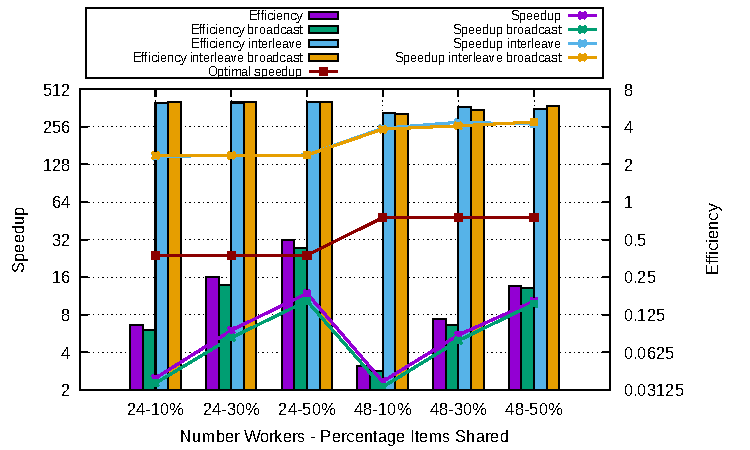
\includegraphics[width=0.45\textwidth]{../logs/scripts/bubble-sort-speedup-efficiency.pdf}
	\caption{Speedup x Efficiency}
	\label{fig:bubble-sort-speedup-efficiency}
\end{figure}

When we used 31 workers, each worker had to sort subvectors with 62500 items. Of these workers, at least 7 of them had to be executed using hyper-threading. In addition, we used the other 9 idle cores. These two facts can explain the 83x increase in speedup when using 31 workers instead of 15.

Forcing cores to use time-sharing for some workers has also increased the speedup for the bubble sort algorithm. However, time-sharing reduced the efficiency, as expected, since workers have to wait for preemption to execute their task on the CPU.

The explanation for this high speedup, even when using time-sharing, may come from the nature of the bubble sort algorithm. Bubble sort has a time complexity of $O(n^2)$ for the worst case scenario. Compared to other sorting algorithms, such as quicksort, the time complexity is the same for the worst case scenario. However, bubble sort algorithm is much less complex. This means that smaller subvectors tend to be sorted faster in bubble sort.

Hence, even with the highest message traffic when more workers are used, the subvectors are sorted faster. This fact also shows that most of the processing time of each worker is spent in sorting the subvector. The merge phase and the sending of messages between the child and parent nodes do not have a major impact on the execution time.

\onecolumn

\section*{Bubble Sort Source Code}
\lstinputlisting[caption=Dataset generator,style=cppStyle]{../bubble-sort/dataset-generator.cpp}
\lstinputlisting[caption=Bubble Sort Sequential,label=lst:bubble-sort-sequential,style=cppStyle]{../bubble-sort/sort-seq.cpp}
\lstinputlisting[caption=Bubble Sort MPI,label=lst:bubble-sort-mpi,style=cppStyle]{../bubble-sort/sort-mpi.cpp}

\end{document}
